%@+leo-ver=5-thin
%@+node:jegc.20110930171547.1123: * @file alternativa.tex
%@@language latex

\documentclass{beamer}

%@+<<tema de beamer>>
%@+node:jegc.20110930171547.1114: ** <<tema de beamer>>
\useinnertheme[shadow=true]{rounded}
\useoutertheme{infolines}
\usecolortheme{orchid}
\definecolor{rojo}{rgb}{0.9,0,0}
\setbeamercolor{structure}{fg=rojo}
\setbeamercolor{item projected}{use=item,fg=black,bg=item.fg!50}
\setbeamercolor*{palette primary}{fg=white,bg=rojo}
\setbeamercolor*{palette secondary}{parent=palette primary,use=palette primary,bg=palette primary.bg!90!black}
\setbeamercolor*{palette tertiary}{parent=palette primary,use=palette primary,bg=palette primary.bg!80!black}
\setbeamercolor*{palette quaternary}{parent=palette primary,use=palette primary,bg=palette primary.bg!70!black}
\setbeamercolor{titlelike}{parent=palette primary}
\setbeamercovered{highly dynamic}
%@-<<tema de beamer>>

\usepackage[utf8]{inputenc}
\usepackage[spanish]{babel}
\usepackage{graphicx}
\usepackage{url}
\usepackage{times}
\usepackage[T1]{fontenc}
\hypersetup{pdfkeywords=open free design source hardware colombia Software Libre abierto 2011 AltaImpedancia alta impedancia electrónica alternativa}

\title[Alternativas para electrónica]{Software Libre una alternativa para soluciones en el campo de la electrónica}
\author[JEGC 2011]{Jorge~Ernesto~Guevara~Cuenca}
\institute[\url{www.altaimpedancia.org}]
{ \inst{1}
  Colibri - Comunidad de Usuarios de Software Libre en Colombia\\
  \url{http://www.slcolombia.org}
  \and
  \inst{2}
  Alta Impedancia - \url{http://www.altaimpedancia.org}
  \and
  \inst{3}
  Hackbo - Hackerspace Bogotá -  \url{http://www.hackbo.co}
  \and
  \inst{4}
  Universidad Autónoma de Colombia - \url{http://www.fuac.edu.co}
}
\date[Semana de Ingeniería FESSJ]
{Semana de Ingeniería\\Fundación de Educación Superior San José\\30 de septiembre de 2011}

\subject{Software Libre una alternativa para soluciones en el campo de la electrónica, Semana de Ingeniería Fundación de Educación Superior San José, 30 de septiembre de 2011}

\logo{
\includegraphics[height=1cm]{img/altaimpedancia}}

\AtBeginSubsection[]
{ \begin{frame}<beamer>{Agenda}
    \tableofcontents[currentsection,currentsubsection]
  \end{frame}}

\beamerdefaultoverlayspecification{<+->}

\begin{document}

\begin{frame}
  \titlepage
\end{frame}

\begin{frame}
  \frametitle{Agenda}
  \tableofcontents
  % You might wish to add the option [pausesections]
\end{frame}

\section<presentation>*{Software Libre una alternativa para la electrónica}

\begin{frame}
  \frametitle{Objetivos}
  \begin{itemize}
  \item Dar a conocer algunas aplicaciones de Software Libre EDA.
  \item Incentivar el uso de Software Libre para electrónica en la educación.
  \end{itemize}
\end{frame}

\section{Proyectos de Open Source Hardware}

\subsection{Motivación}

%\subsection<presentation>*{Nivel de restricción}

\begin{frame}{Openmoko}{\url{http://www.openmoko.com}}
  \begin{figure}
    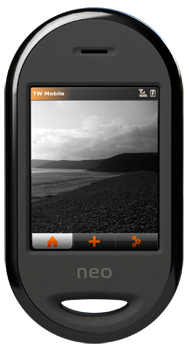
\includegraphics[scale=0.65]{img/freerunner_shop1}
    \caption{Teléfono móvil.}
    \label{fig:openmoko}
  \end{figure}
\end{frame}

\begin{frame}{The Open Graphics Project}{\url{http://opengraphics.org}}
  \begin{figure}
    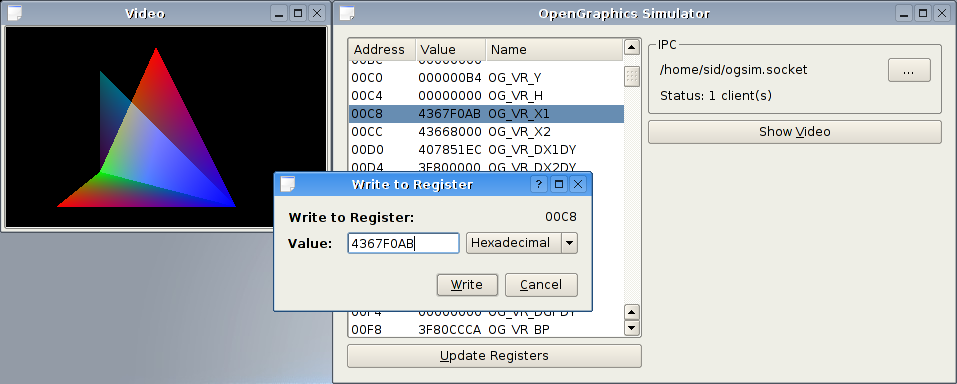
\includegraphics[scale=0.35]{img/ogsim-screen1}
    \caption{Tarjeta de video.}
    \label{fig:ogp}
  \end{figure}
\end{frame}

\begin{frame}{Open sparc}{\url{http://www.opensparc.net}}
  \begin{figure}
    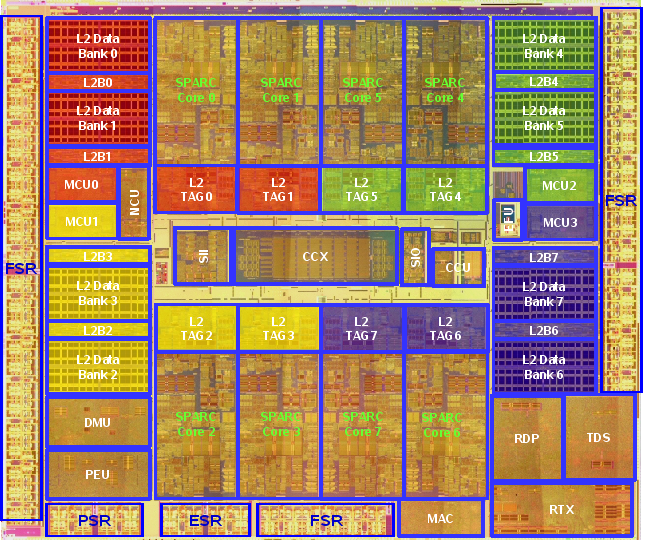
\includegraphics[scale=0.4]{img/ultrasparc-t2-layout}
    \caption{Procesador de 64 bits.}
    \label{fig:opensparc}
  \end{figure}
\end{frame}

\begin{frame}{Ronja}{\url{http://ronja.twibright.com}}
  \begin{figure}
    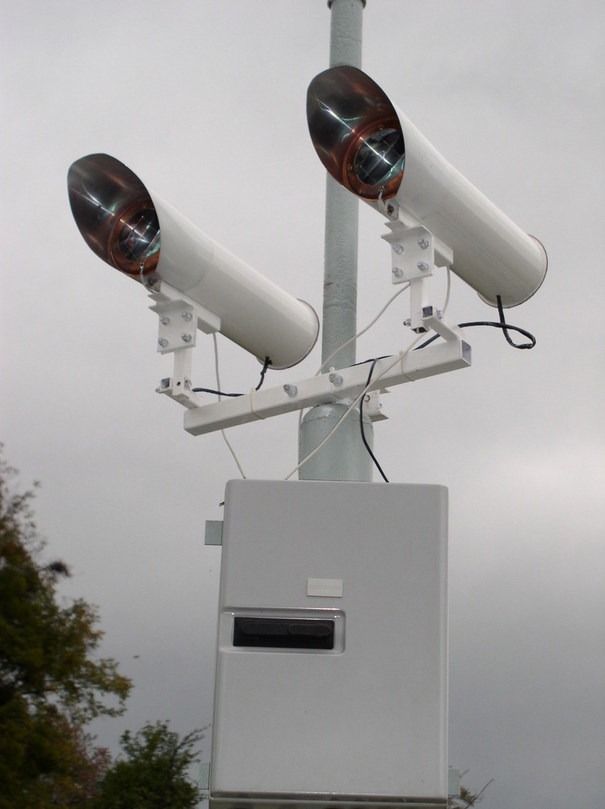
\includegraphics[scale=0.22]{img/122e}
%    \caption{Nivel de restricción 0}
    \label{fig:ronja}
  \end{figure}
\end{frame}

\begin{frame}{RobotCub}{\url{http://www.robotcub.org}}
  \begin{figure}
    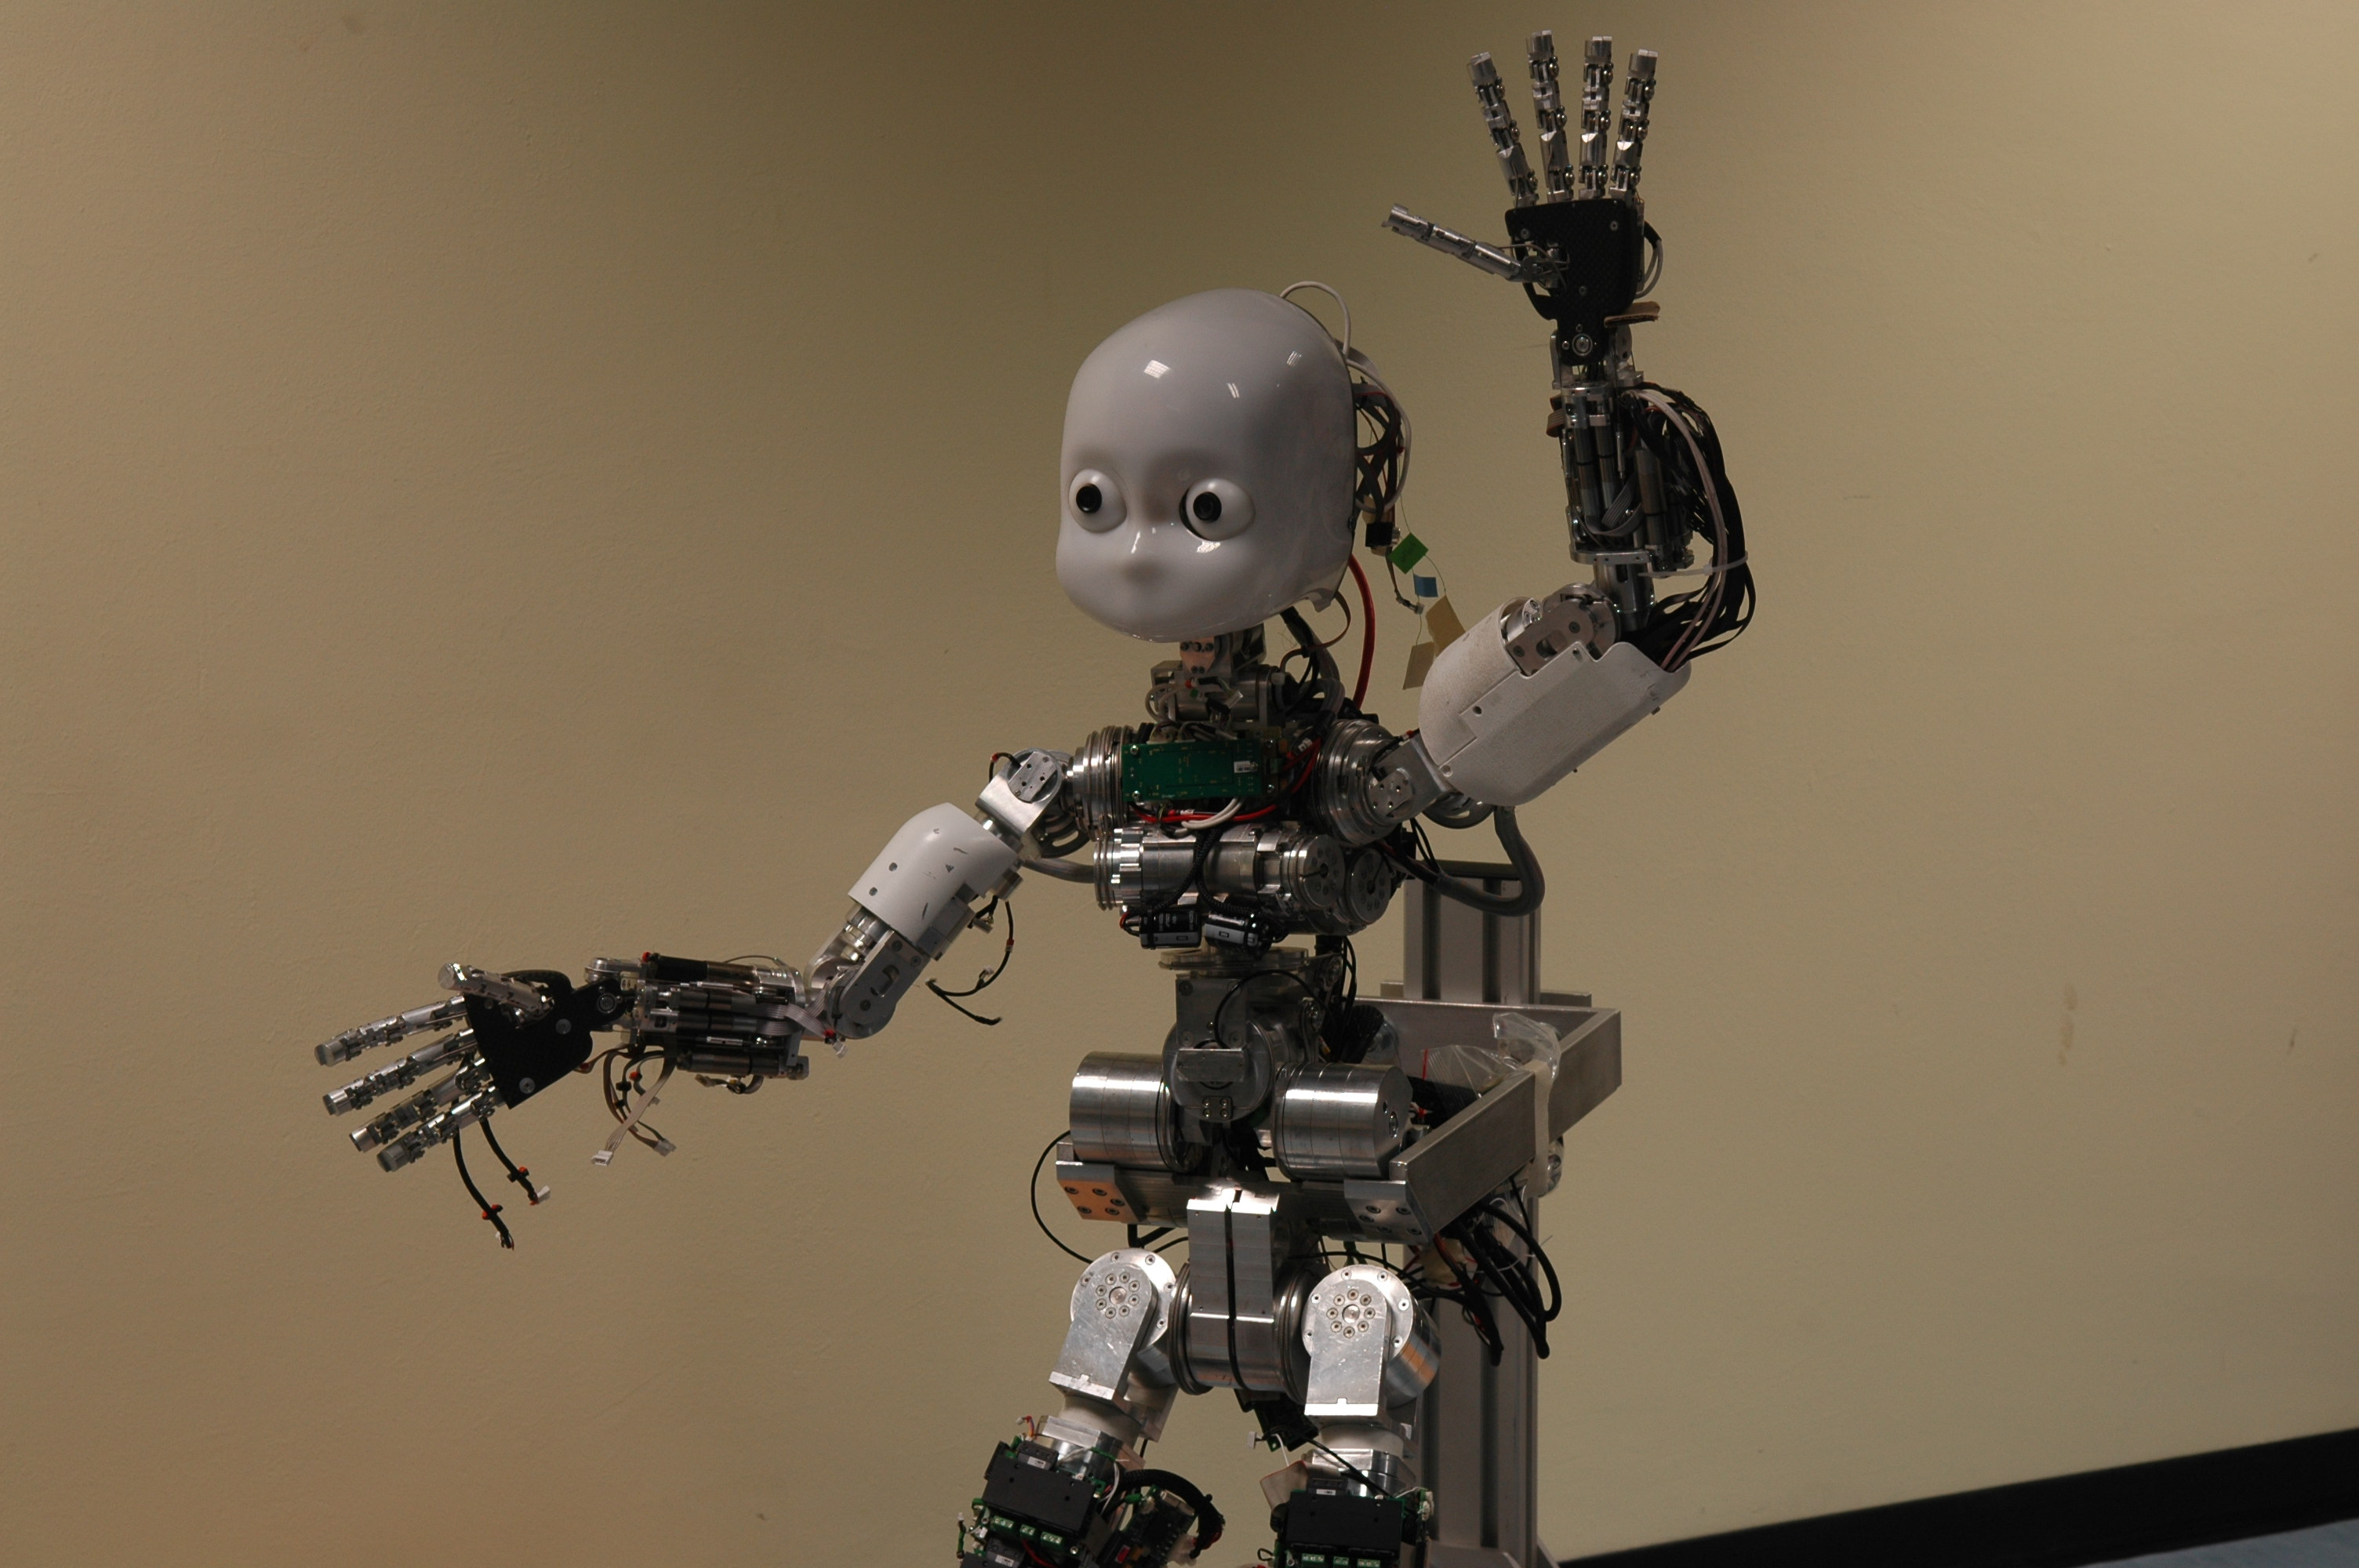
\includegraphics[scale=0.085]{img/DSC_3997}
    \caption{iCub.}
    \label{fig:icub}
  \end{figure}
\end{frame}

\begin{frame}{ECB AT91 V2}{\url{http://www.emqbit.com}}
  \begin{figure}
    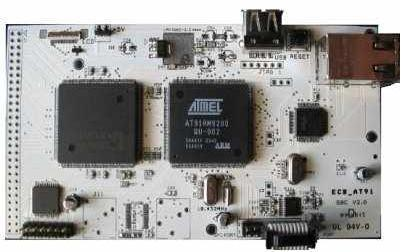
\includegraphics[scale=0.6]{img/V2}
    \caption{Free open SBC design Single Board.}
    \label{fig:ecb}
  \end{figure}
\end{frame}

\begin{frame}{Arduino}{\url{http://www.arduino.cc}}
  \begin{figure}
    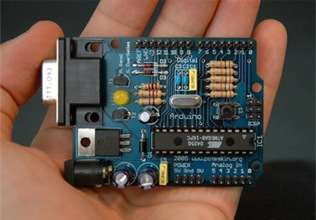
\includegraphics[scale=0.6]{img/arduino316}
    \caption{Plataforma para prototipado.}
    \label{fig:arduino}
  \end{figure}
\end{frame}

% gnuradio http://gnuradio.org/trac/wiki/USRP
% VoIP http://www.rowetel.com/ucasterisk/index.html

\section{Como se hace el hardware}

\subsection{Lo que se necesita}

\begin{frame}{Herramientas EDA}{¿Qué es CAD?}
  \begin{itemize}
  \item CAD es el acrónimo de Computer Aided Design (Diseño asistido por computador).
  \item En principio se refiere a aplicaciones para hacer dibujos.
  \item Se usa en general para cualquier campo del conocimiento en el que se pueda diseñar por medio de un computador.
  \item ECAD es el acrónimo de Electronic Computer Aided Design (Diseño electrónico asistido por computador).
  \end{itemize}
\end{frame}

\begin{frame}{Herramientas EDA}{¿Qué es EDA?}
  \begin{itemize}
  \item EDA es el acrónimo de Electronic Design Automation (Automatización de diseño electrónico).
  \item Se refiere a todas las herramientas involucradas en el desarrollo de hardware.
  \item Es todo el software ECAD y hardware requeridos para el desarrollo de hardware.
  \item Hardware requerido
    \begin{itemize}
    \item HDK (Hardware Development Kits)
    \item HPP (Hardware Prototyping Plataforms).
    \end{itemize}
  \end{itemize}
\end{frame}

\begin{frame}{Herramientas EDA}
  \begin{itemize}
  \item Lenguajes de descripción de circuitos.
    \begin{itemize}
    \item netlist, ejemplo spice.
    \item HDL, ejemplo verilog.
    \end{itemize}
    \vspace{9pt}
  \item Captura esquemática y modelado gráfico.
    \begin{itemize}
    \item Diagramas de flujo.
    \item ASM.
    \item etc\dots{}
    \end{itemize}

    \vspace{9pt}
  \item Simuladores y visualizadores.
    \vspace{9pt}
  \item Fabricación de tarjetas de cirtuitos impresos (PCB).
  \item Fabricación de circuitos integrados (VLSI).
  \item Programación de dispositivos lógicos (FPGA, PAL, PLD).
  \end{itemize}
\end{frame}

\subsection{Como se hace}

\begin{frame}
  \begin{figure}
    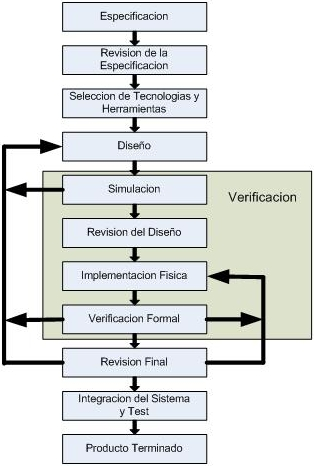
\includegraphics[scale=0.6]{img/metodologia}
    \caption{Metodología universal de diseño \cite{Guillermo}.}
    \label{fig:metodologia}
  \end{figure}
\end{frame}

\subsection{Lo que se obtiene}

\begin{frame}{Producto terminado}
  \begin{figure}
    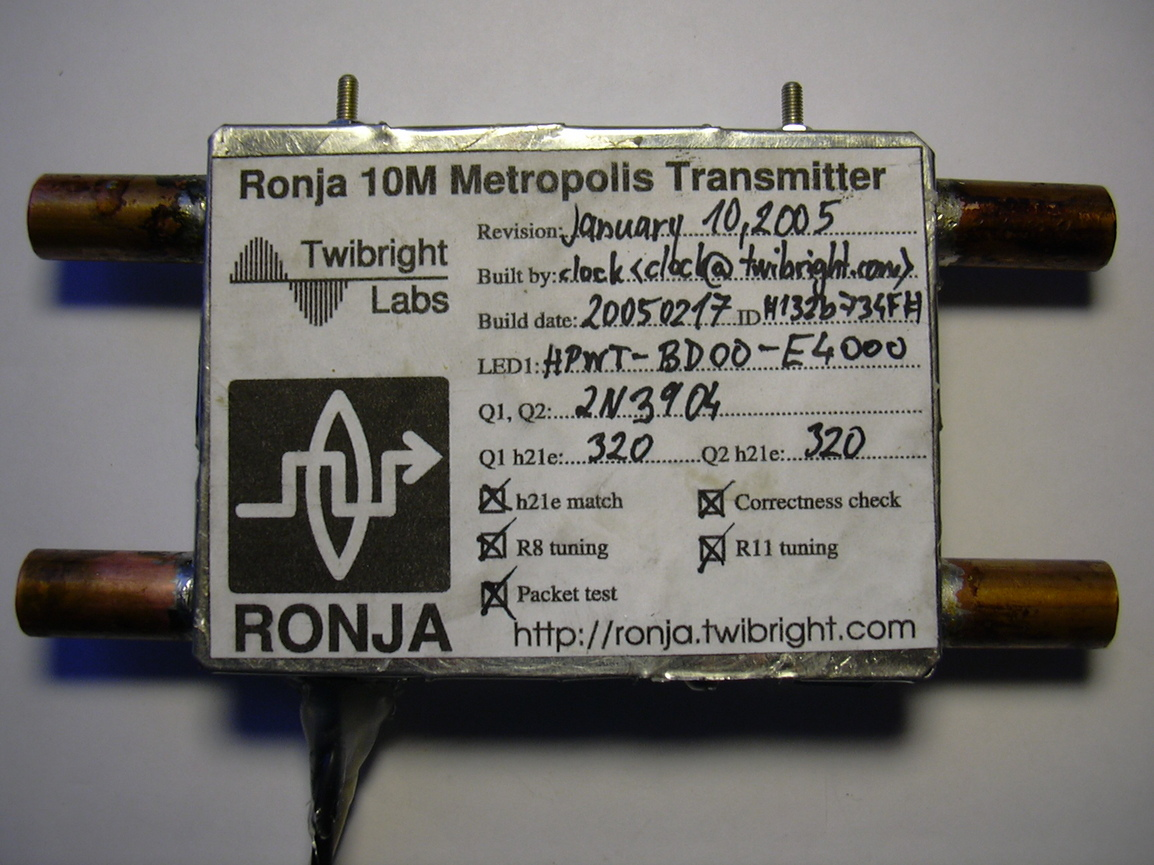
\includegraphics[scale=0.85]{transmisor/1b80}
    \caption{Transmisor Ronja 10M Metropolis}
  \end{figure}
\end{frame}

\begin{frame}{Hardware mecánico}
  \begin{figure}
    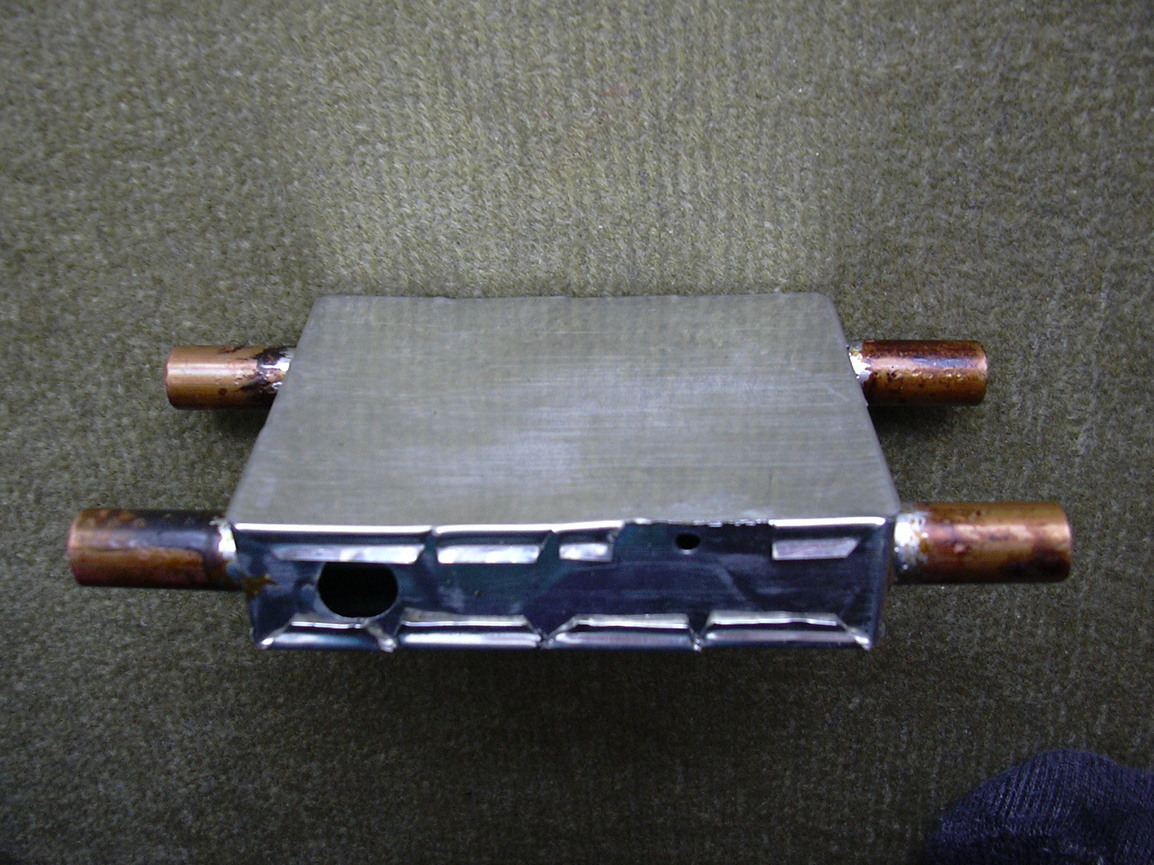
\includegraphics[scale=0.9]{transmisor/1b50}
  \end{figure}
\end{frame}

\begin{frame}{Diseño Hardware mecánico}{Hecho en \textbf{qcad} - \url{http://www.ribbonsoft.com/qcad_downloads.html}}
  \begin{figure}
    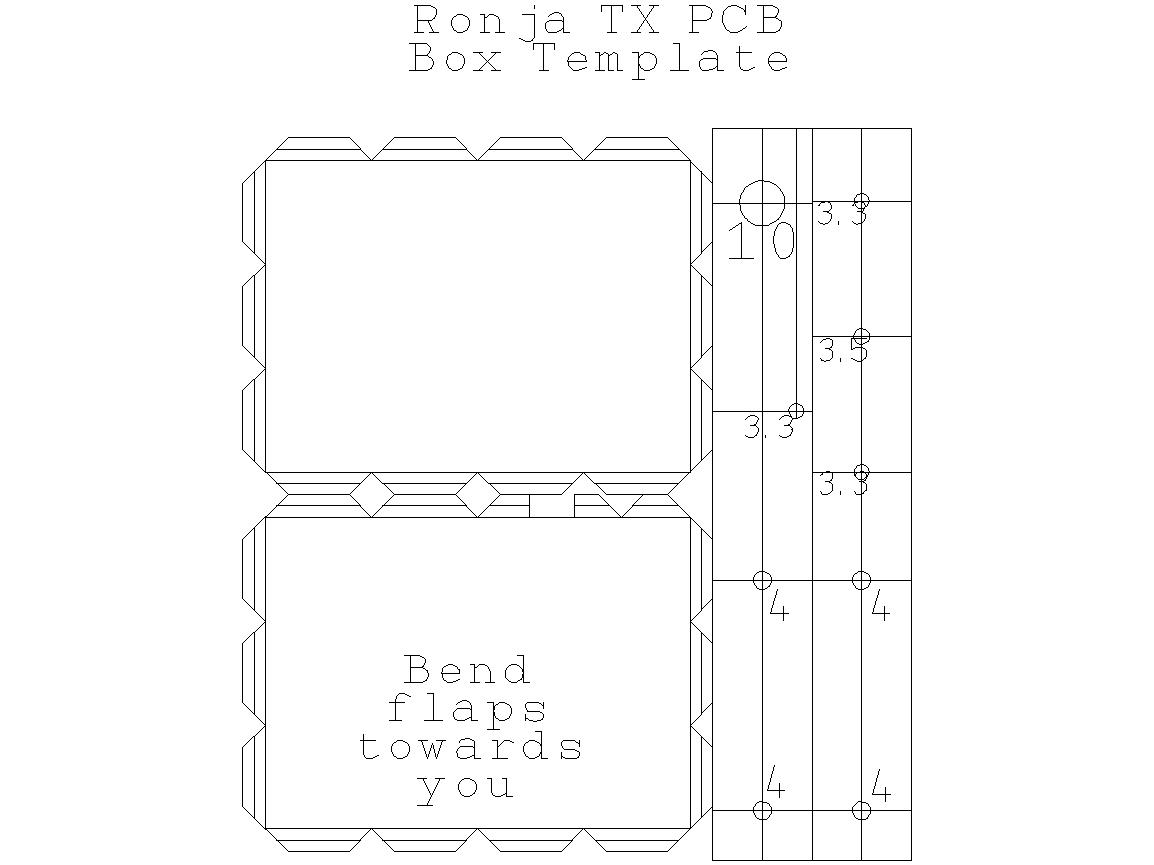
\includegraphics[scale=0.225]{transmisor/tx_pcb2}
  \end{figure}
\end{frame}

\begin{frame}{Hardware mecánico}
  \begin{figure}
    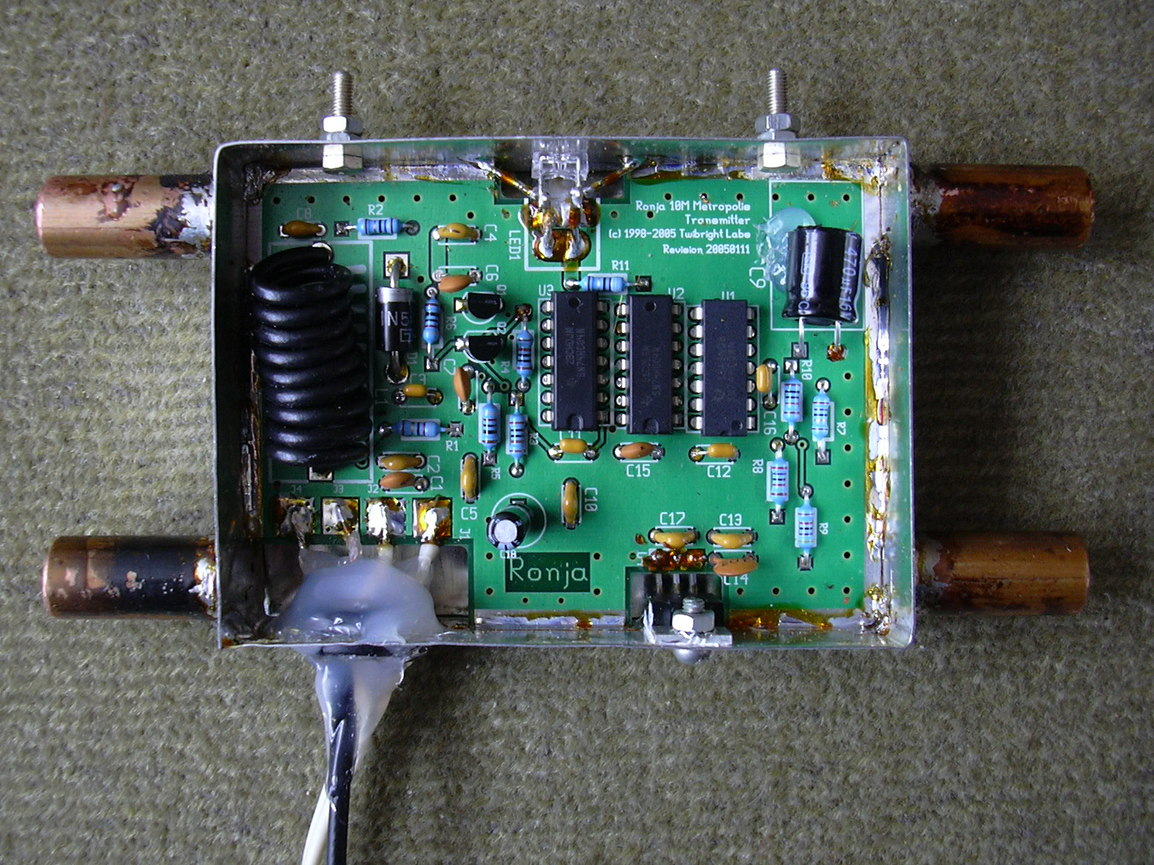
\includegraphics[scale=0.85]{transmisor/1b76}
    \caption{Dentro esta el Hardware electrónico}
  \end{figure}
\end{frame}

\begin{frame}{Hardware electrónico}
  \begin{figure}
    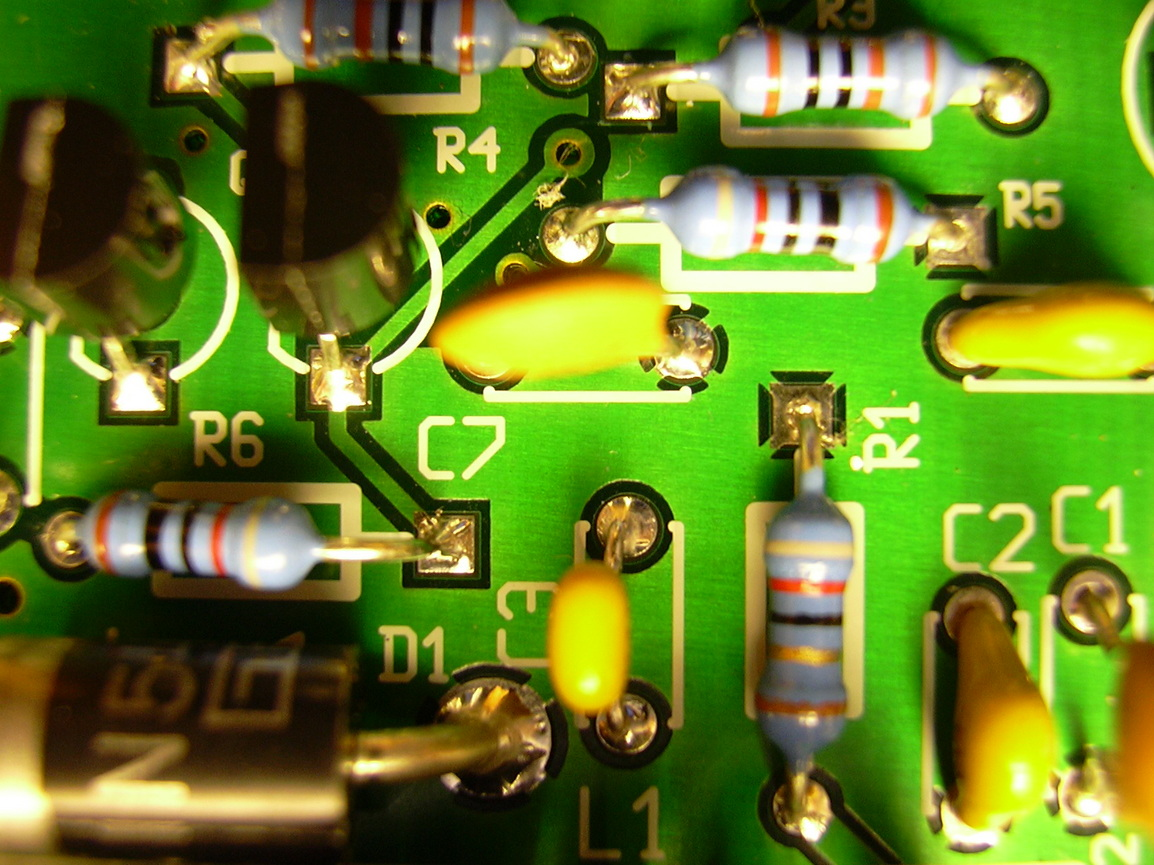
\includegraphics[scale=0.85]{transmisor/1b84}
    \caption{Tarjeta con dispositivos electrónicos}
  \end{figure}
\end{frame}

\begin{frame}{Hardware electrónico}
  \begin{figure}
    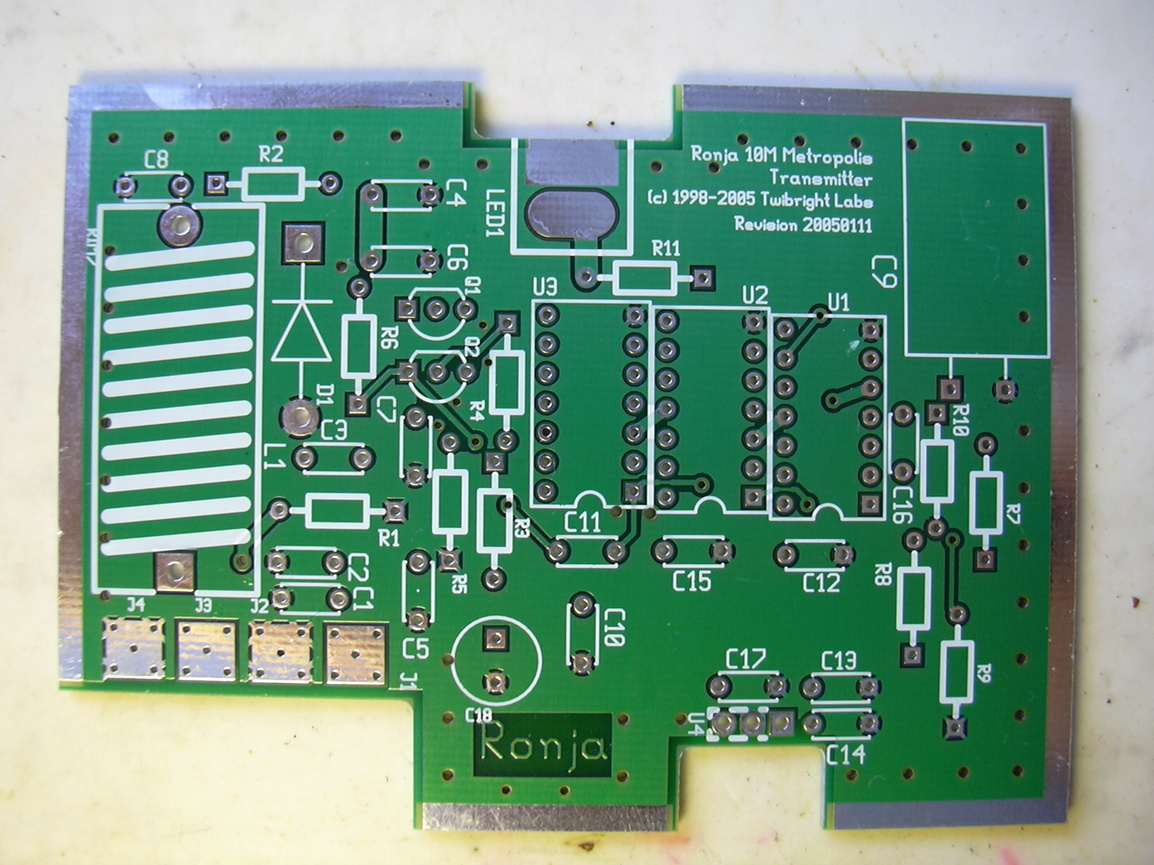
\includegraphics[scale=0.85]{transmisor/1b5e}
    \caption{Tarjeta de circuito impreso (PCB)}
  \end{figure}
\end{frame}

\begin{frame}{Hardware electrónico}{Se visualiza con \textbf{gerbv} - \url{http://gerbv.sourceforge.net}}
  \begin{figure}
    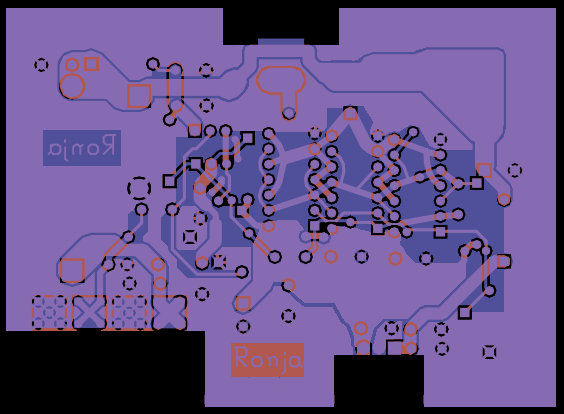
\includegraphics[scale=0.4]{transmisor/transmisor_gerber.png}
    \caption{Archivo gerber}
  \end{figure}
\end{frame}

\begin{frame}{Diseño de Hardware electrónico}{Se edita con \textbf{pcb} - \url{http://pcb.gpleda.org}}
  \begin{figure}
    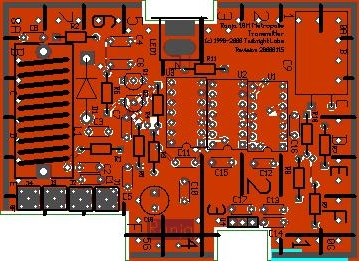
\includegraphics[scale=0.65]{transmisor/metropolis_transmitter}
    \caption{Archivo PCB}
  \end{figure}
\end{frame}

\begin{frame}{Diseño de Hardware electrónico}{Creado con \textbf{gEDA/gschem} - \url{http://www.gpleda.org}}
  \begin{figure}
    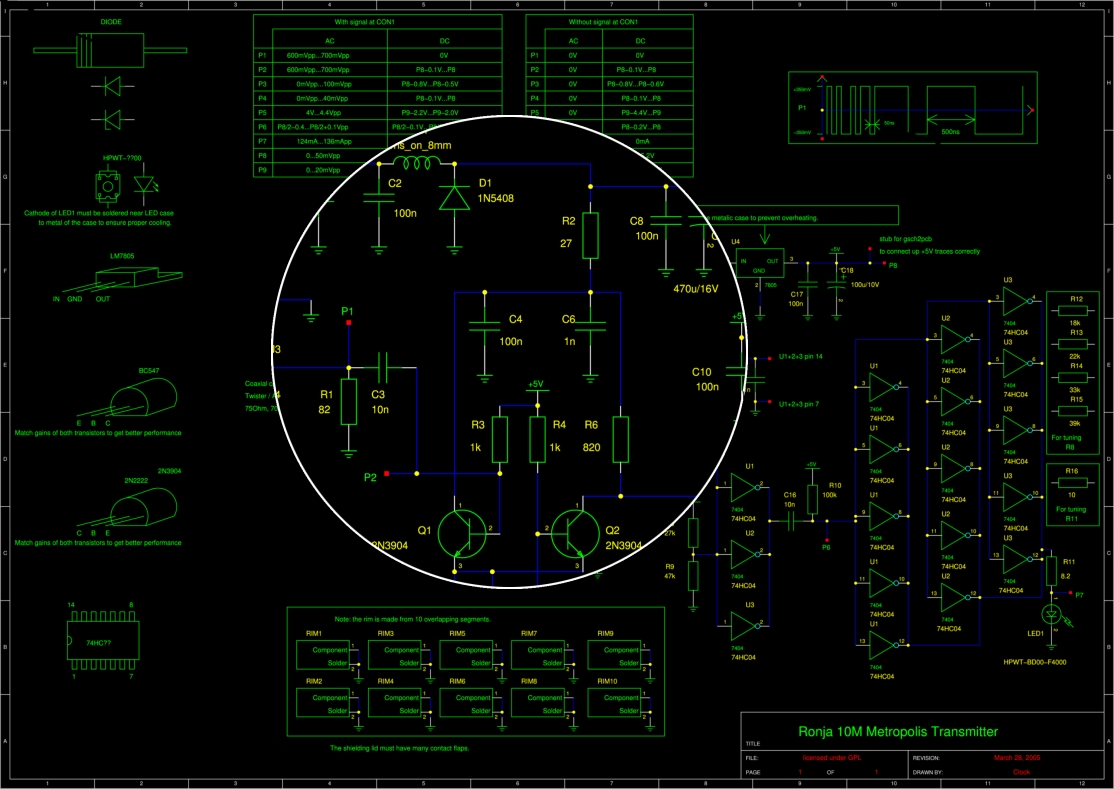
\includegraphics[scale=0.21]{transmisor/transmisor_esquema}
    \caption{Archivo del diagrama esquemático}
  \end{figure}
\end{frame}

\section{Software Libre disponible}

\subsection[gEDA - \url{http://www.gpleda.org}]{gEDA}

%ynetlist http://ynetlist.sourceforge.net/

\begin{frame}{gEDA}{GPL'd Electronic Design Automation}
  \begin{figure}[!h]
    \centering
    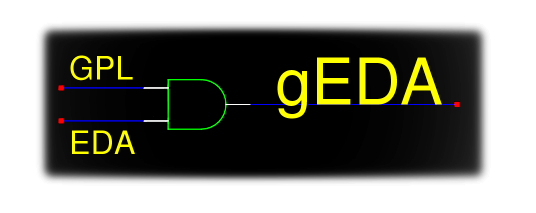
\includegraphics[scale=0.4]{img/geda.png}
  \end{figure}
  \begin{itemize}
  \item gEDA es acrónimo de GPL'd Electronic Design Automation.
  \item gEDA es una suite de aplicaciones de software libre EDA para diseño de circuitos eléctricos, con la que se puede hacer captura esquemática, simulación, creación de prototipos y producción.
  \end{itemize}
\end{frame}

\begin{frame}{gEDA}{Herramientas que componen la suite}
  \begin{itemize}
  \item gEDA / gaf(gschem and friends)
      \begin{itemize}
      \item Captura esquemática.
      \item Librería de símbolos.
      \item Verificador de símbolos.
      \item Editor de atributos.
      \item Generador de netlist.
      \item Utilidades.
      \item Documentación y ejemplos.
      \end{itemize}
    \item Desarrolladas separadamente pero que se usan con la suite.
      \begin{itemize}
      \item Simulación análoga.
      \item Creación de circuitos impresos.
      \item Simulación digital.
      \end{itemize}
  \end{itemize}
\end{frame}

% \begin{frame}{gaf - gschem and friends}{gschem}
%   \begin{figure}[!h]
%     \centering
%     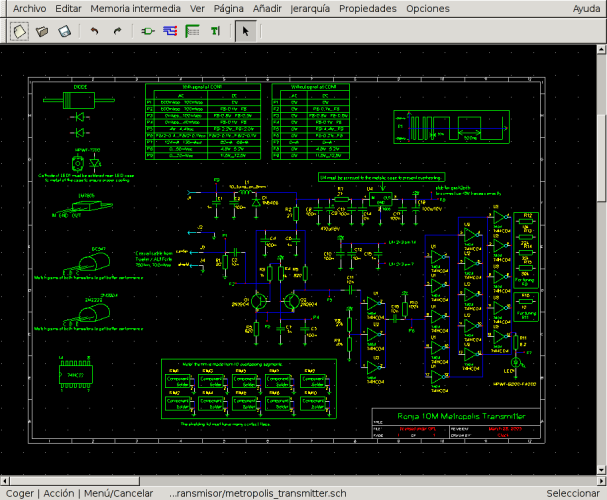
\includegraphics[scale=0.35]{img/gscheme.png}
%   \end{figure}

% \end{frame}

% \begin{frame}{gaf - gschem and friends}{gschem}
%   Programa de dibujo especializado para ECAD.
%   \begin{itemize}
%   \item Entiende conexiones eléctricas.
%   \item Asociación de atributos.
%   \item Diseño jerárquico.
%   \item Programado en C y scheme.
%   \end{itemize}
% \end{frame}

\begin{frame}{gaf - gschem and friends}{Librería de símbolos}
  \begin{figure}[!h]
    \centering
    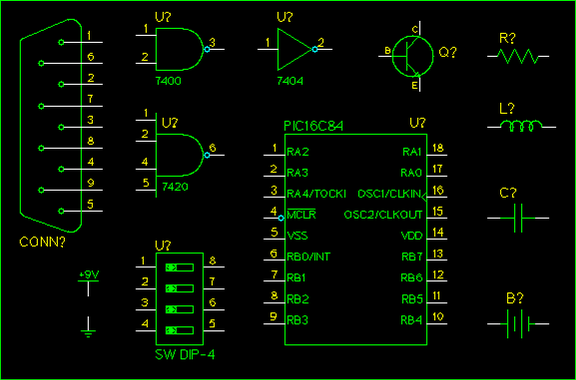
\includegraphics[scale=0.25]{img/simbolos.png}
  \end{figure}
  \begin{itemize}
  \item Más de 1400 símbolos, todos bajo GPL.
  \item El formato de archivo es ASCII, usado para símbolos y esquemas.
  \item Descarga de símbolos \url{http://www.gedasymbols.org}
  \item \textbf{gsymcheck} Verificador de símbolos.
  \end{itemize}
\end{frame}

\begin{frame}{gaf - gschem and friends}{gattrib}
  \begin{figure}[!h]
    \centering
    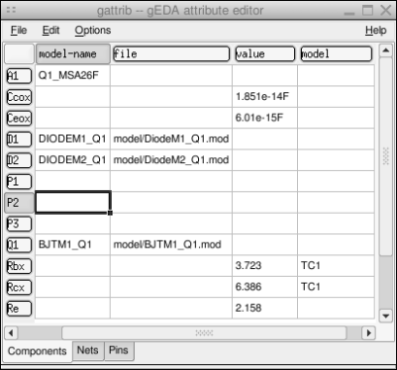
\includegraphics[scale=0.4]{img/gattrib.png}
  \end{figure}
  Editor de Atributos
\end{frame}

\begin{frame}{gaf - gschem and friends}{docs, examples}
  \begin{itemize}
  \item \textbf{gnetlist} Genera apartir de archivo esquemático un netlist en alguno de los 28 formatos soportados.
    \pause
  \item Utilidades: 17 utilidades más que complementan gEDA/gaf (cli).
    \begin{itemize}
    \item gmk\_sym, smash\_megafile, convert\_sym, sarlacc\_schem, olib, gsch2pcb, grenum, gschlas, sarlacc\_sym, gschupdate, gsymupdate, gschemdoc, refdes\_renum, tragesym, pads\_backannotate, garchive, gsymfix.pl
    \end{itemize}
  \end{itemize}
\end{frame}

\begin{frame}{gaf - gschem and friends}{docs, examples}
  \begin{itemize}
  \item Documentación: Manuales de los programas y el wiki completo hasta la fecha de la revisión.
    \pause
  \item Ejemplos:
    \begin{itemize}
    \item gTAG: Interface para conectar desde el puerto USB del computador a dispositivos conm JTAG.
    \item Detector de luz
    \item Amplificador de radio frecuencia
    \item Amplificador en dos etapas
    \end{itemize}
  \end{itemize}
\end{frame}

\begin{frame}{Simulación análoga}{\textbf{gnucap} - \url{http://www.gnu.org/software/gnucap}}
  GNU circuit Analisys Package
  \begin{itemize}
  \item Simulador de circuitos de proposito general.
  \item Aunque soporta modelos de spice no esta basado en spice.
  \end{itemize}
\end{frame}

\begin{frame}{Simulación análoga}{\textbf{ngspice} - \url{http://ngspice.sourceforge.net}}
  \begin{figure}[!h]
    \centering
    
\includegraphics[scale=0.5]{img/nglogo.jpg}
  \end{figure}
  Simulador de circuitos basado en los simuladores de código abierto Spice3f5, Cider1b1 y Xspice.
\end{frame}

\begin{frame}{Simulación análoga}{GSpiceUI}
  \begin{figure}[!h]
    \centering
    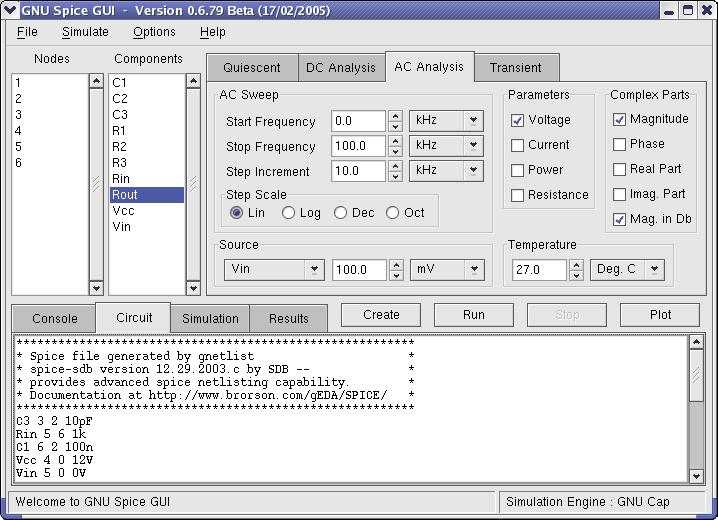
\includegraphics[scale=0.3]{img/GSpiceUI.jpg}
  \end{figure}
  Frontend gráfico para gnucap y ngspice.
\end{frame}

\begin{frame}{Simulación análoga}{\textbf{gwave} - \url{http://gwave.sourceforge.net}}
  \begin{figure}[!h]
    \centering
    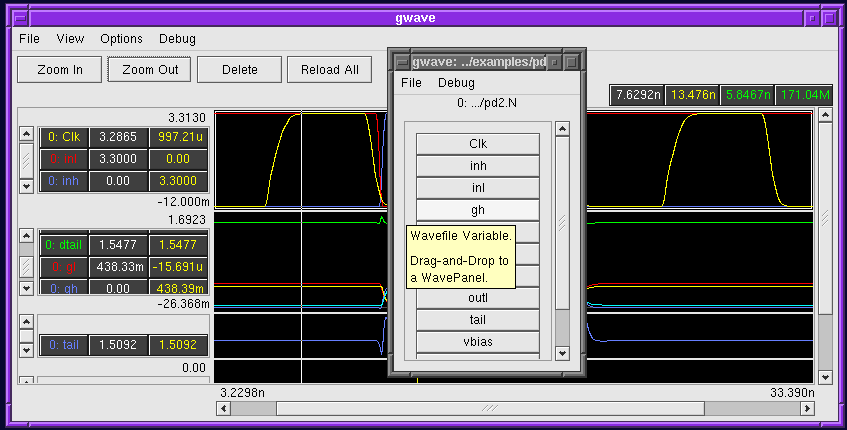
\includegraphics[scale=0.25]{img/gwave.png}
  \end{figure}
  \begin{itemize}
  \item Visor de señales análogas.
  \item Puede leer archivos bianrios (raw) de spice2G6, spice3F5 o ngspice y datos tabulados en formato ASCII para usar con gnucap o cualquier otra herramienta que genere este tipo de archivo.
  \end{itemize}
\end{frame}

\begin{frame}{Creación de circuitos impresos}{xgsch2pcb}
  \begin{figure}[!h]
    \centering
    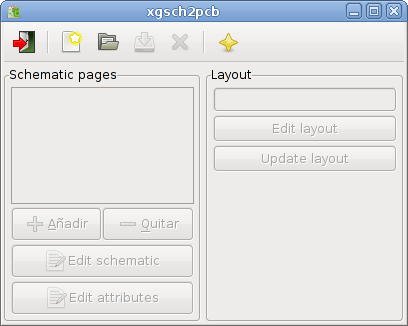
\includegraphics[scale=0.35]{img/xgsch2pcb.png}
  \end{figure}
  Front-end gráfico para generar archivos pcb apartir de un archivo de gschem.
\end{frame}

% \begin{frame}{Creación de circuitos impresos}{PCB - \url{http://pcb.gpleda.org}}
%   \begin{figure}[!h]
%     \centering
%     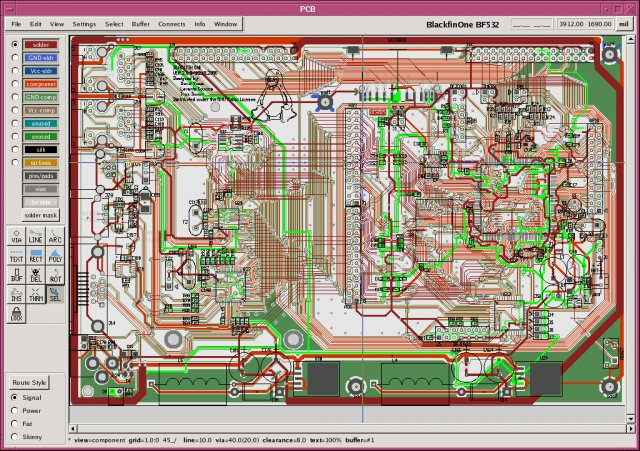
\includegraphics[scale=0.35]{img/pcb.jpg}
%   \end{figure}
%   Editor de circuitos impresos (PCB).
% \end{frame}

% \begin{frame}{Creación de circuitos impresos}{Gerbv - \url{http://gerbv.sourceforge.net}}
%   \begin{figure}[!h]
%     \centering
%     
\includegraphics{img/gerbv.png}
%   \end{figure}
%   Visor de archivos gerber.
% \end{frame}

\begin{frame}{Simulación digital}{Icarus Verilog - \url{http://www.icarus.com/eda/verilog}}
  \begin{figure}[!h]
    \centering
    
\includegraphics[scale=0.6]{img/icarus.png}
  \end{figure}
  \textbf{iverilog} Herramienta de simulación y síntesis para el lenguaje de descripción de hardware Verilog HDL.
\end{frame}

\begin{frame}{Simulación digital}{\textbf{gtkwave} - \url{http://gtkwave.sourceforge.net}}
  \begin{figure}[!h]
    \centering
    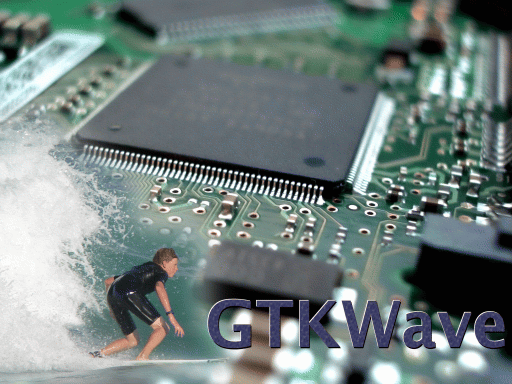
\includegraphics[scale=0.25]{img/gtkwave.png}
  \end{figure}
  \begin{itemize}
  \item Visor de señales digitales.
  \item Formatos soportados: VCD, EVCD,	LXT, Synopsis y .out.
  \end{itemize}
\end{frame}

% \begin{frame}{Simulación digital}{\textbf{vhdl2vl} - \url{http://doolittle.icarus.com/~larry/vhd2vl}}
%   \begin{itemize}
%   \item Traductor de código sintetizable en VHDL a Verilog HDL.
%     \pause
%   \item \textbf{wcalc} Herramienta para análisis y síntesis de estructuras de líneas de transmision y componentes relacionados.
%   \end{itemize}
% \end{frame}

\subsection[Simuladores de circuitos]{Simuladores de circuitos}

\begin{frame}{Oregano}{\url{http://arrakis.gforge.lug.fi.uba.ar}}
  \begin{figure}[!h]
    \centering
    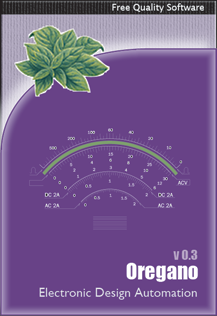
\includegraphics[scale=0.3]{img/oregano.png}
  \end{figure}
  Oregano es una aplicación de GNOME para la captura y la impresión de esquemas de circuitos electrónicos. Puede simular los circuitos usando Gnucap, ng-spice o spice de Berkeley.
\end{frame}

\begin{frame}{Qucs - Quite Universal Circuit Simulator}{\url{http://qucs.sourceforge.net}}
  \begin{figure}[!h]
    \centering
    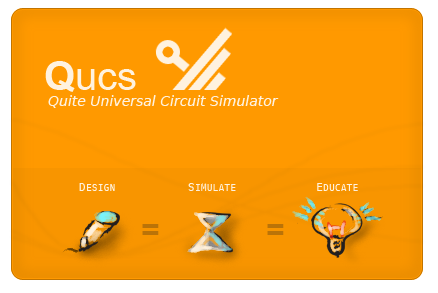
\includegraphics[scale=0.3]{img/qucslogo4.png}
  \end{figure}
  \begin{itemize}
  \item Simulador de circuitos bastante universal.
  \item Qucs es un simulador de circuitos integrado, lo que significa que puede configurar un circuito eléctrico con un interfaz gráfico y simular su comportamiento en pequeña señal, gran señal y con ruido.
  \end{itemize}
\end{frame}

\subsection[PCB]{Herramientas para el diseño de circuitos impresos}

\begin{frame}{kicad}{\url{http://kicad.sourceforge.net}}
  \begin{figure}[!h]
    \centering
    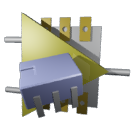
\includegraphics[scale=0.5]{img/kicad.png}
  \end{figure}
  KiCad consiste en un gestor de proyectos y cuatro programas principales.
\end{frame}

% \begin{frame}{kicad}{El gestor de proyectos}
%   \begin{figure}[!h]
%     \centering
%     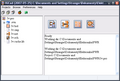
\includegraphics{img/kicad-project.png}
%   \end{figure}
%   \textbf{kicad} Permite crear y nombrar proyectos e iniciar la mayor parte de los componentes de KiCad.
% \end{frame}

% \begin{frame}{kicad}{El editor de esquemas}
%   \begin{figure}[!h]
%     \centering
%     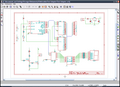
\includegraphics{img/eeschema.png}
%   \end{figure}
%   \textbf{eeschema} Permite crear y nombrar proyectos e iniciar la mayor parte de los componentes de KiCad.
% \end{frame}

% \begin{frame}{kicad}{El selector de componentes usados en el diseño del circuito}
%   \textbf{cvpcb} Es una herramienta que permite asignar huellas/formas (footprint) de circuito impreso a los símbolos esquemáticos del diseño en eeschema.
% \end{frame}

% \begin{frame}{kicad}{El programa editor de circuitos impresos}
%   \begin{figure}[!h]
%     \centering
%     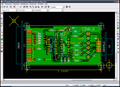
\includegraphics{img/pcbnew.png}
%   \end{figure}
%   \textbf{pcbnew} Contiene el editor de módulos (representación gráfica de la forma/huella), donde se pueden cambiar y crear los módulos.
% \end{frame}

% \begin{frame}{kicad}{El visor Gerber (Documentos de Fotoploter)}
%   \begin{figure}[!h]
%     \centering
%     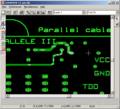
\includegraphics{img/gerbview.png}
%   \end{figure}
%   \textbf{gerbview} Visor Gerber para verificar los archivos gerber (son los archivos .pho en KiCad), que es el formato de archivos que generalmente solicitan los fabricantes de circuitos impresos.
% \end{frame}

\begin{frame}{liquidpcb}{\url{http://www.liquidpcb.org}}
  \begin{figure}[!h]
    \centering
    
\includegraphics[scale=0.4]{img/liquidpcb.png}
  \end{figure}
  Herramienta para el diseño de circuitos impresos.
  \begin{figure}[!h]
    \centering
    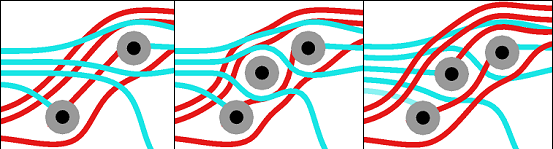
\includegraphics[scale=0.5]{img/flexi.png}
  \end{figure}
\end{frame}

\subsection{Simuladores de circuitos digitales}

\begin{frame}{tkgate}{\url{http://www.tkgate.org}}
  \begin{figure}[!h]
    \centering
    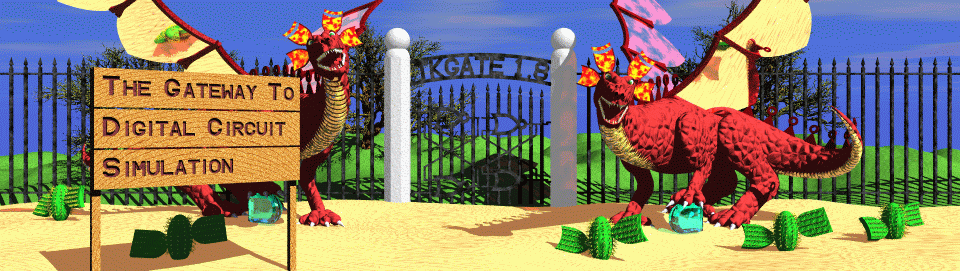
\includegraphics[scale=0.35]{img/tkgate.png}
  \end{figure}
  Simulador de circuitos digitales
\end{frame}

\begin{frame}{klogic}{\url{http://www.a-rostin.de}}
  \begin{figure}[!h]
    \centering
    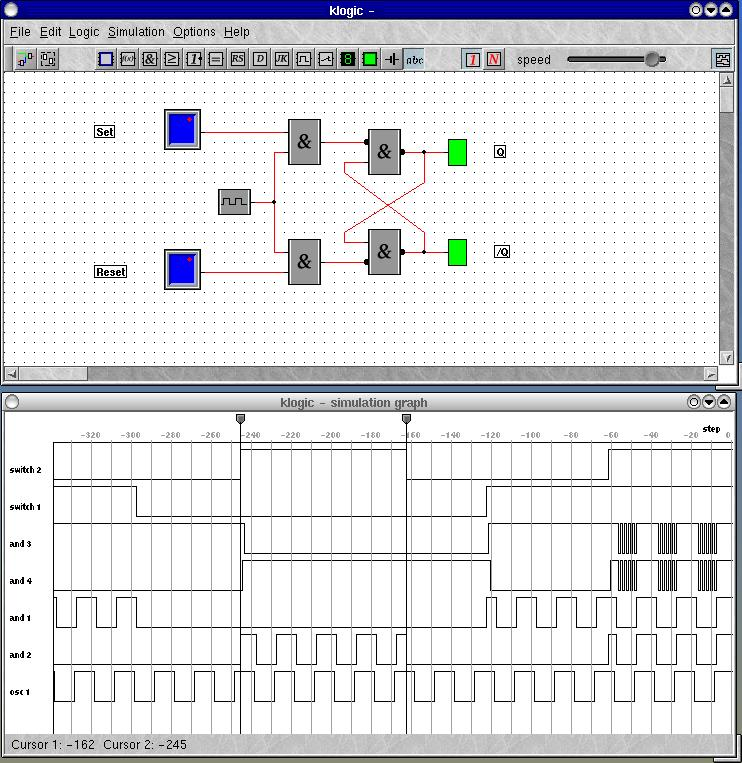
\includegraphics[scale=0.18]{img/klogic.jpg}
  \end{figure}
  KLogic es una aplicación para construir y simular circuitos digitales fácilemnte.
\end{frame}

\subsection[Microcontroladores]{Software para desarrollo con microcontroladores}

\begin{frame}{AVR de Atmel}{Compiladores de C}
  \begin{figure}[!h]
    \centering
    
\includegraphics[scale=2]{img/atmel_logo.jpg}
  \end{figure}
  \begin{itemize}
  \item SDCC - Small Device C Compiler (Compilador de C para dispositivos pequeños). \url{http://sdcc.sourceforge.net}
  \item gcc-avr - GNU C compiler (compilador cruzado para AVR)
  \item avr-libc - Biblioteca estándar de C de desarrollo para AVR de Atmel.
  \end{itemize}
\end{frame}

\begin{frame}{AVR de Atmel}{AVRA}
  \begin{figure}[!h]
    \centering
    
\includegraphics[scale=2]{img/atmel_logo.jpg}
  \end{figure}
  Ensamblador para microcontroladores AVR de Atmel.
  \url{http://avra.sourceforge.net}
\end{frame}

\begin{frame}{AVR de Atmel}{SimulAVR - \url{http://www.nongnu.org/simulavr}}
  \begin{figure}[!h]
    \centering
    
\includegraphics[scale=0.5]{img/simulavr_logo.png}
  \end{figure}
  SimulAVR simula la familia de microcontroladores AVR de Atmel, emula un objetivo remoto de gdb, y muestra información de registros y memoria en tiempo real.
\end{frame}

\begin{frame}{AVR de Atmel}{Depuradores}
  \begin{figure}[!h]
    \centering
    
\includegraphics[scale=2]{img/atmel_logo.jpg}
  \end{figure}
  \begin{itemize}
  \item AVaRICE - Traduce entre el protocolo de depuración remota de GDB y el protocolo JTAG ICE de AVR.
  \item gdb-avr - The GNU Debugger (El depurador de GNU para AVR)
  \end{itemize}
\end{frame}

\begin{frame}{AVR de Atmel}{Programadores}
  \begin{itemize}
  \item AVRDUDE - AVR Downloader/UploaDEr (Software para programar los microcontroladores AVR de Atmle). \url{http://www.nongnu.org/avrdude}.
  \item UISP - AVR In-System Programmer (Programador In-System para AVR). \url{http://www.nongnu.org/uisp}
  \item avrp - Software para utilizar con los programadores de Atmel utilizando el estándar de comunicación para puerto serial. \url{http://tihlde.org/~jonah/el/avrp.html}
  \end{itemize}
\end{frame}

\begin{frame}{AVR de Atmel}{Programadores}
  \begin{itemize}
  \item s51dude - Herramienta de programación In-System específicamente diseñada para ser utilizada con la tarjeta usbtinyisp y la familia de microcontroladores Atmel de 8051. \url{http://s51dude.gforge.lug.fi.uba.ar}
  \item DFU-programer es un actualizador de firmware de dispositivos basados en programación USB para los chips Atmel con bootloader USB. \url{http://dfu-programmer.sourceforge.net}
  \end{itemize}
 \end{frame}

\begin{frame}{AVR de Atmel}{Varios}
  \begin{itemize}
  \item ppc-evtd - A simple and small user-space interface daemon to the Linkstation/Kuro AVR micro-controller found in embedded NASes. \url{http://sourceforge.net/projects/ppc-evtd}
  \item ava - Algebraical Virtual Assembler for Atmel's AVR MCUs
  \end{itemize}
\end{frame}

\begin{frame}{PIC de Microchip}{Ensambladores}
  \begin{itemize}
  \item  gputils - GNU PIC Utilities (Utilidades para la familia de microcontroladores PIC de Microchip). \url{http://gputils.sourceforge.net}
  \item  picasm - Un ensamblador para la familia de microcontroladores PIC de Microchip. Es válido para la mayoría de la familia de PIC de Microchip. Usa la sintaxis de Microchip (no Parallax). \url{http://www.jmp.fi/~trossi/pic}
  \item  PTK4L (PIC ToolKit for Linux) es un conjunto de ensamblador, desensamblador y programador de microcontroladores PIC16C84 y PIC16F84. \url{http://www.rastersoft.com/ptk4l.htm}
  \end{itemize}
\end{frame}

\begin{frame}{PIC de Microship}{Simuladores - Gpsim}
  \begin{figure}[!h]
    \centering
    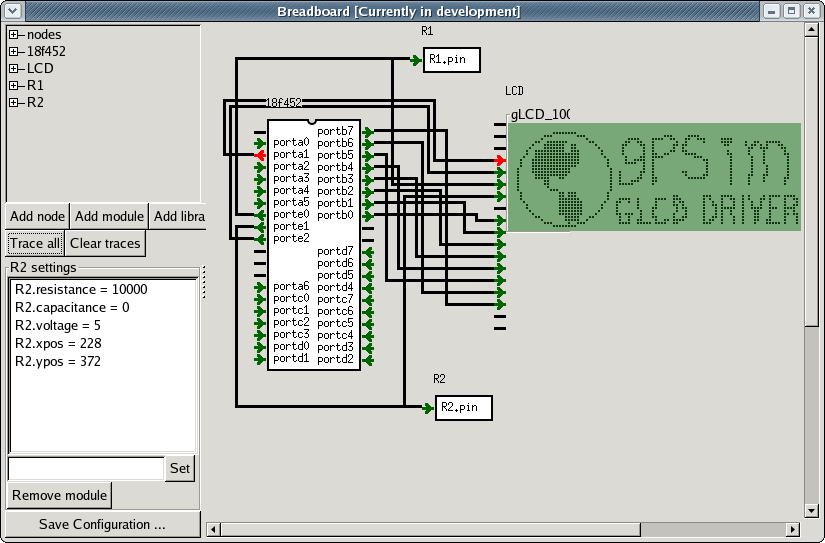
\includegraphics[scale=0.2]{img/gpsim.png}
  \end{figure}
  Gpsim es un simulador de software con todas las funcionalidades de los microcontroladores PIC de Microchip. \url{http://gpsim.sourceforge.net}
\end{frame}

\begin{frame}{PIC de Microship}{Simuladores}
  \begin{itemize}
  \item simulpic - Simulador para el microcontrolador PIC16F84. \url{http://alumni.media.mit.edu/~deva/software.shtml}
  \item nitpic - Simulador para el microcontrolador PIC16C84.
  \end{itemize}
\end{frame}

\begin{frame}{PIC de Microship}{Programadores - PICPROG}
    \begin{figure}[!h]
    \centering
    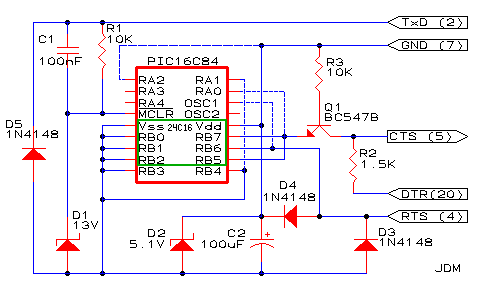
\includegraphics[scale=0.4]{img/picprog.png}
  \end{figure}
  Software para programar por el puerto serial microcontroladores PIC de Microchip. \url{http://hyvatti.iki.fi/~jaakko/pic/picprog.html}
\end{frame}

\begin{frame}{PIC de Microship}{Programadores - PICP}
  \begin{figure}[!h]
    \centering
    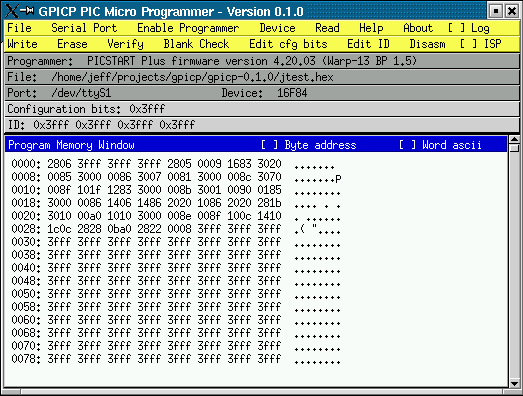
\includegraphics[scale=0.3]{img/gpicp.png}
  \end{figure}
  Utilidad que permite el uso de programadores PICSTART o compatibles. \url{http://home.pacbell.net/theposts/picmicro}  
\end{frame}

\begin{frame}{PIC de Microship}{Programadores - PIC USB Framework}
  \begin{figure}[!h]
    \centering
    
\includegraphics[scale=0.25]{img/vasco.png}
  \end{figure}
  Framework de aplicación USB dedicado a Linux (del lado del host) y a la familia de microcontroladores PIC18F4550 (del lado del dispositivo). \url{http://vasco.gforge.enseeiht.fr}
  \begin{itemize}
  \item \textbf{odyssey} - Aplicación para programar microcontroladores PIC de Microchip. \url{http://vasco.gforge.enseeiht.fr/index.php?article=Odyssey.html} 
  \end{itemize}
\end{frame}

\begin{frame}{PIC de Microship}{IDE's}
  \begin{itemize}
  \item piklab
    \begin{itemize}
    \item pikloops
    \end{itemize}
  \item pikdev
  \item ktechlab
  \item yapide \url{http://www.mtoussaint.de/yapide.html}
  \end{itemize}
\end{frame}

% \subsection[Diseño VLSI]{Herramientas para diseño VLSI}

% % \begin{frame}{Open Circuit Design}{\url{http://www.opencircuitdesign.com}}
% %   \begin{figure}[!h]
% %     \centering
% %     \includegraphics[scale=0.5]{img/opencircuit.png}
% %   \end{figure}
% %   Suite de software de fuente abierta EDA
% % \end{frame}

% % \begin{frame}{Open Circuit Design}{Herramientas}
% %   \begin{figure}[!h]
% %     \centering
% %     \includegraphics[scale=0.4]{img/magic.png}
% %   \end{figure}
% %   Herramienta de diseño VLSI
% %   \begin{figure}[!h]
% %     \centering
% %     \includegraphics[scale=0.4]{img/xcircuit.png}
% %   \end{figure}
% %   Capturador esquemático
% % \end{frame}

% % \begin{frame}{Open Circuit Design}{Herramientas}{IRSIM}
% %   \begin{figure}[!h]
% %     \centering
% %     \includegraphics[scale=0.3]{img/analyzer.png}
% %   \end{figure}
% %   Simulador de circuitos digitales.
% % % irsim-mode http://code.google.com/p/irsim-mode/
% % \end{frame}

% % \begin{frame}{Open Circuit Design}{Herramientas}
% %   \begin{itemize}
% %   \item \textbf{netgen} Es una herramienta para comparar netlists, un proceso conocido como LVS, que significa "Diseño vs Esquema".
% %   \item PCB: El mismo programa para diseño de pcbs usado por gEDA.
% %   \end{itemize}
% % \end{frame}

% \begin{frame}{electric}{\url{http://www.staticfreesoft.com}}
%   \begin{figure}[!h]
%     \centering
%     \includegraphics[scale=0.5]{img/electric.jpg}
%   \end{figure}
%   Sistema EDA completo para diseño VLSI
%   \begin{itemize}
%   \item Captura esquemática.
%   \item Diseño CMOS.
%   \item Maneja HDL's: Verilog VHDL
%   \item PLD's
%   \end{itemize}
% \end{frame}

% \begin{frame}{alliance}{\url{http://www-asim.lip6.fr/recherche/alliance}}
%   \begin{figure}[!h]
%     \centering
%     \includegraphics[scale=0.5]{img/alliancelogo.png}
%   \end{figure}
%   Conjunto de herramientas CAD y librerias para diseño VLSI
%   \begin{itemize}
%   \item Compilador y simulador de VHDL.
%   \item Herramientas de síntesis.
%   \item Herramientas de "Place and route" (asignación y enrrutado).
%   \end{itemize}
% \end{frame}

% \begin{frame}{toped}{\url{http://www.toped.org.uk}}
%   \begin{figure}[!h]
%     \centering
%     \includegraphics[scale=0.3]{img/toped.png}
%   \end{figure}
%   Editor de diseño de Circuitos Integrados
% \end{frame}

% \subsection{Herramientas para desarrollo con HDLs}

% \begin{frame}
%   \begin{itemize}
%   \item ghdl
%   \item freehdl
%   \item myhdl
%   \end{itemize}
% %IVI
% \end{frame}
% \begin{frame}{veripool}{\url{http://www.veripool.org}}
%   \begin{itemize}
%   \item Dinotrace
%   \item Verilator
%   \item Verilog-Mode
%   \item Verilog-Perl
%   \item mas...
%   \end{itemize}
% \end{frame}

% % \subsection{Otros}

% % \begin{frame}{ksimus}
  
% % \end{frame}

% % \begin{frame}
% % gnetman - Gnetman es principalmente un traductor netlists, capaz de convertir entre formatos como VHDL, Verilog y SPICE.
% % MUCS-PCB - http://intranet.cs.man.ac.uk/apt/projects/tools/mucs-pcb/
% % pyastra http://pyastra.sourceforge.net/
% % usbprog - \url{http://developer.berlios.de/projects/usbprog}
% % openocd - \url{http://openocd.berlios.de}
% % atcl - Arbitrary Transmission Line Calculator
% % qmc
% % eqntott http://code.google.com/p/eqntott/
% % editores
% %  emacs modo vhdl  
% % \end{frame}

% % \subsection{out of date}

% % \begin{frame}
% %  ViPEC http://vipec.sourceforge.net/index.html
% %  Tclspice http://tclspice.sourceforge.net/
% %  Chipmunk tools http://www.cs.berkeley.edu/~lazzaro/chipmunk/pickup/pickup.html
% %  gael  
% % \end{frame}


% % \begin{frame}{Laboratorio}
% % qtdmm http://www.mtoussaint.de/qtdmm.html
% % xoscope http://xoscope.sourceforge.net/
% % http://goodfet.sourceforge.net/
% % \end{frame}

\subsection{Herramienta para documentar}

\begin{frame}{\LaTeX}
  \begin{itemize}
  \item Documentación estructurada (WYSIWYM - What You See Is What You Mean)
  \item Paquetes especializados
    \begin{itemize}
    \item Mapas de karnaugh
    \item Formatos IEEE
    \item Esquemas de circuitos
    \item Muchos más\dots
    \end{itemize}

  \end{itemize}
\end{frame}

\begin{frame}{cirkuit}{\url{http://wwwu.uni-klu.ac.at/magostin/cirkuit.html}}
  \begin{figure}
    \includegraphics[scale=0.35]{img/cirkuit1.png}
  \end{figure}
\end{frame}

\section<presentation>*{Software Libre una alternativa para la electrónica}

\begin{frame}{¿Que tiene que ver Debian en esta charla?}
  \begin{figure}
    \includegraphics[scale=0.32]{img/choice.jpg}
  \end{figure}
    \begin{itemize}
  \item También existe FEL
  \end{itemize}
\end{frame}

\begin{frame}{Conclusión}
  \begin{block}{}
    Hay suficiente software EDA libre disponible, entonces la tarea es empezar a usarlo en las aulas de clase y compartir las experiencias.
  \end{block}
\end{frame}

\appendix

\section<presentation>*{Referencias}

\begin{frame}
  \frametitle<presentation>{Bibliografía}
  \begin{thebibliography}{99}
    \beamertemplatebookbibitems
  \bibitem[1]{PardoBoluda}Fernando Pardo Carpio y José A. Boluda Grau
    \newblock \emph{VHDL, Lenguaje para síntesis y modelado de circuitos, 2a. edición}
    \newblock Alfaomega, 2004
  \end{thebibliography}
\end{frame}

\begin{frame}
  \frametitle<presentation>{Bibliografía}
  \begin{thebibliography}{99}
    \beamertemplatearticlebibitems
  \bibitem<1->[Güichal 2005]{Guillermo}Guillermo Güichal
    \newblock \emph{Diseño Digital Utilizando Lógicas Programables}
    \newblock Junio 29, 2005
    \newblock \url{http://fpga.com.ar/notas/NotasCompletas.pdf}
  \end{thebibliography}
\end{frame}

\begin{frame}
  \frametitle<presentation>{Infografía}
  \begin{thebibliography}{99}
    \beamertemplatearticlebibitems
  \bibitem[5]{Ales}\emph{gEDA - GPL Electronic Design Automation}, \url{http://www.geda.seul.org/talks/deluge_ales.pdf}
  \bibitem<1->[6]{ronja}\emph{Ronja 10M Metropolis Transmitter}, \url{http://ronja.twibright.com/transmitter/index.php}
    % \item Charlas de Fredy y Jorge
  \end{thebibliography}
\end{frame}

\section<presentation>*{Sobre este documento}

\begin{frame}
  \begin{block}{Licencia}
    \begin{figure}
      \includegraphics[scale=0.9]{img/by-sa}
    \end{figure}
    \centering
    \small Creative Commons\\
    \small Atribución-Compartir Obras Derivadas Igual 2.5 Colombia\\
    \small \url{http://creativecommons.org/licenses/by-sa/2.5/co}
\end{block}
\begin{block}{}
  Creado con \LaTeX / Beamer
\end{block}
\end{frame}

\section<presentation>*{Comunidades}

\begin{frame}{Como unirse}
  \begin{figure}
    \includegraphics{img/altaimpedancia-acerca-de}
  \end{figure}
  \begin{block}{}
    \begin{itemize}
    \item Linux en Caja - \url{http://linuxencaja.net}
    \item HackBo - \url{http://hackbo.co}
    \end{itemize}
  \end{block}
  \begin{block}{Contacto}
    \centering
    Jorge Ernesto Guevara Cuenca\\
    \href{mailto:ernesto@altaimpedancia.org}{ernesto@altaimpedancia.org}\\
  \end{block}
\end{frame}


\end{document}
%@-leo
